%%%%%%%%%%%%%%%%%%%%%%%%%%%%%%%%%%%%%%%%%
% Beamer Presentation
% LaTeX Template
% Version 1.0 (10/11/12)
%
% This template has been downloaded from:
% http://www.LaTeXTemplates.com
%
% License:
% CC BY-NC-SA 3.0 (http://creativecommons.org/licenses/by-nc-sa/3.0/)
%
%%%%%%%%%%%%%%%%%%%%%%%%%%%%%%%%%%%%%%%%%

%----------------------------------------------------------------------------------------
% PACKAGES AND THEMES
%----------------------------------------------------------------------------------------

\documentclass{beamer}

\mode<presentation> {

% The Beamer class comes with a number of default slide themes
% which change the colors and layouts of slides. Below this is a list
% of all the themes, uncomment each in turn to see what they look like.

%\usetheme{default}
%\usetheme{AnnArbor}
%\usetheme{Antibes}
%\usetheme{Bergen}
%\usetheme{Berkeley}
%\usetheme{Berlin}
%\usetheme{Boadilla}
%\usetheme{CambridgeUS}
%\usetheme{Copenhagen}
%\usetheme{Darmstadt}
%\usetheme{Dresden}
%\usetheme{Frankfurt}
%\usetheme{Goettingen}
%\usetheme{Hannover}
%\usetheme{Ilmenau}
%\usetheme{JuanLesPins}
%\usetheme{Luebeck}
\usetheme{Madrid}
%\usetheme{Malmoe}
%\usetheme{Marburg}
%\usetheme{Montpellier}
%\usetheme{PaloAlto}
%\usetheme{Pittsburgh}
%\usetheme{Rochester}
%\usetheme{Singapore}
%\usetheme{Szeged}
%\usetheme{Warsaw}

% As well as themes, the Beamer class has a number of color themes
% for any slide theme. Uncomment each of these in turn to see how it
% changes the colors of your current slide theme.

%\usecolortheme{albatross}
%\usecolortheme{beaver}
%\usecolortheme{beetle}
%\usecolortheme{crane}
%\usecolortheme{dolphin}
%\usecolortheme{dove}
%\usecolortheme{fly}
%\usecolortheme{lily}
%\usecolortheme{orchid}
%\usecolortheme{rose}
%\usecolortheme{seagull}
%\usecolortheme{seahorse}
\usecolortheme{whale}
%\usecolortheme{wolverine}

%\setbeamertemplate{footline} % To remove the footer line in all slides uncomment this line
%\setbeamertemplate{footline}[page number] % To replace the footer line in all slides with a simple slide count uncomment this line

%\setbeamertemplate{navigation symbols}{} % To remove the navigation symbols from the bottom of all slides uncomment this line
}

% \usepackage[pdftex]{graphicx}
% \graphicspath{{../pdf/}{../jpeg/}}
% \DeclareGraphicsExtensions{.pdf,.jpeg,.png}
\usepackage[brazil]{babel}
\usepackage[utf8]{inputenc}
\usepackage[T1]{fontenc}
\usepackage{amsmath}
\usepackage{amssymb}
\usepackage{mathabx}
\usepackage{algorithmic}
\usepackage{array}
\usepackage{float}
\usepackage{mdwmath}
\usepackage{mdwtab}
\usepackage{eqparbox}
\usepackage{url}
\usepackage{graphicx} % Allows including images
\usepackage{booktabs} % Allows the use of \toprule, \midrule and \bottomrule in tables

\setbeamertemplate{itemize items}[ball]

%----------------------------------------------------------------------------------------
% TITLE PAGE
%----------------------------------------------------------------------------------------

\title[]{Projeto de Controladores por Alocação de Polos\\Aplicados a um Sistema de Suspensão Ativa} % The short title appears at the bottom of every slide, the full title is only on the title page

\author[Joacy Mesquita, Márcia Prado]{Orientando: Joacy Mesquita da Silva\\Orientadora: Márcia Lissandra Machado Prado} % Your name
\institute[UEFS] % Your institution as it will appear on the bottom of every slide, may be shorthand to save space
{
Trabalho de Conclusão de Curso\\Curso de Engenharia de Computação\\Universidade Estadual de Feira de Santana \\ % Your institution for the title page
\medskip
\textit{joacymsilva@gmail.com, marcia.lissandra@gmail.com} % Your email address
}
\date{03 de agosto de 2018} % Date, can be changed to a custom date

\begin{document}

\begin{frame}
\titlepage % Print the title page as the first slide
\end{frame}

\begin{frame}
\frametitle{Roteiro} % Table of contents slide, comment this block out to remove it
\tableofcontents % Throughout your presentation, if you choose to use \section{} and \subsection{} commands, these will automatically be printed on this slide as an overview of your presentation
\end{frame}

%----------------------------------------------------------------------------------------
% PRESENTATION SLIDES
%----------------------------------------------------------------------------------------

%------------------------------------------------
\section{Introdução} % Sections can be created in order to organize your presentation into discrete blocks, all sections and subsections are automatically printed in the table of contents as an overview of the talk
%------------------------------------------------

\begin{frame}
\frametitle{Introdução}
\begin{itemize}
\item Sistemas de Controle \cite{ogata}, \cite{nise}.
\item Alocação de Polos \cite{ogata}, \cite{maitelli}.
\item Sistema de Suspensão Ativa \cite{quanser}.
\item Objetivo do Trabalho.
\end{itemize}
\end{frame}

% \begin{frame}
% \frametitle{Introdução}
% \begin{itemize}
% \item Sistemas de Controle.
% \item Alocação de Polos.
% \item Sistema de Suspensão Ativa.
% \item Objetivo do Trabalho.
% \end{itemize}
% \end{frame}

\section{Projeto usando Função de Transferência (FT)}
\begin{frame}
\Huge{\centerline{Projeto usando}}
\Huge{\centerline{Função de Transferência}}
\end{frame}
\subsection{Modelagem do Sistema}
\begin{frame}
\frametitle{Função de Transferência: Modelagem do Sistema}
\begin{itemize}
\item Para o projeto, foi utilizado o Sistema de Suspensão Ativa da \textit{Quanser} \cite{quanser}. O modelo físico concedido pelo fabricante se encontra na Figura \ref{suspensao}.
\end{itemize}

\begin{figure}[H]
  \centering
  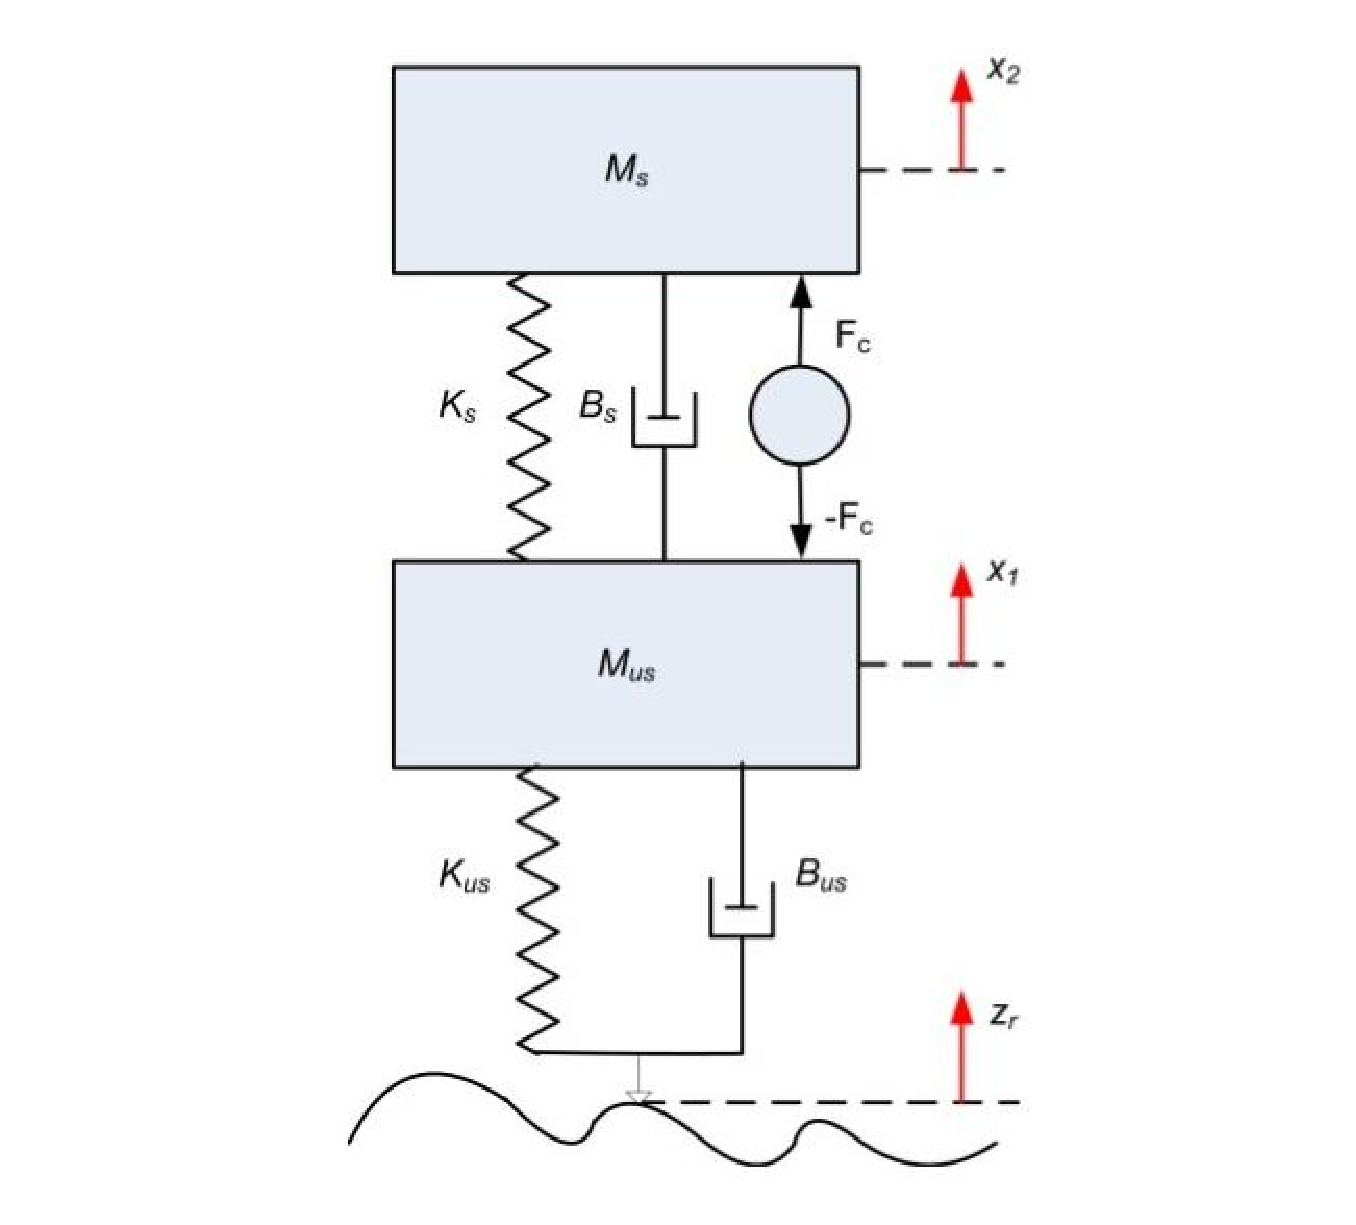
\includegraphics[width=.5\columnwidth]{./imagens/suspensao.pdf}
    \renewcommand{\figurename}{Fig. 1}
  \caption{Modelo para o Sistema de Suspensão Ativa da \textit{Quanser} \protect\cite{quanser}.}
  \label{suspensao}
\end{figure}
\end{frame}

\begin{frame}
\frametitle{Função de Transferência: Modelagem do Sistema}
\begin{itemize}
\item A modelagem matemática foi possível através da representação do sistema em Equações Diferenciais, as Equações (\ref{x2}) e (\ref{x1}) foram obtidas.
\end{itemize}

\begin{equation}\label{x2}
\begin{matrix}
\ddot{x_2} = -g + \frac{F_c}{M_s} + \frac{B_s}{M_s}\dot{x_1} - \frac{B_s}{M_s}\dot{x_2} + \frac{K_s}{M_s}x_1 -\frac{K_s}{M_s}x_2
\end{matrix}
\end{equation}

\begin{equation}\label{x1}
\begin{matrix}
\ddot{x_1}= -g - \frac{F_c}{M_{us}} - \frac{B_s+B_{us}}{M_{us}}\dot{x_1} + \frac{B_{us}}{M_{us}}\dot{x_2} + \frac{B_{us}}{M_{us}}\dot{z_r}\\- \frac{K_s+K_{us}}{M_{us}}x_1 + \frac{K_s}{M_{us}}x_2 + \frac{K_{us}}{M_{us}}z_r
\end{matrix}
\end{equation}
\end{frame}

\begin{frame}
\frametitle{Função de Transferência: Modelagem do Sistema}
\begin{itemize}
\item Os valores numéricos atribuídos a cada parâmetro da Figura \ref{suspensao} são apresentados na Tabela \ref{parametros}.
\end{itemize}

\begin{table}[H]{\centering}
\centering
  \renewcommand{\tablename}{Tabela 1}
  \caption{Parâmetros do Sistema de Suspensão Ativa.}
  \begin{tabular}{|c|c|c|} \hline
   Parâmetro & Valor & Unidade \\ \hline
   $M_s$ & 2,45 & kg \\ \hline
   $M_{us}$ & 1 & kg \\ \hline
   $K_s$ & 900 & N/m \\ \hline
   $K_{us}$ & 1250 & N/m \\ \hline
   $B_s$ & 7,5 & N.s/m \\ \hline
   $B_{us}$ & 5 & N.s/m \\ \hline
   \end{tabular}
  \label{parametros}
\end{table}
\end{frame}

\begin{frame}
\frametitle{Função de Transferência: Modelagem do Sistema}
\begin{itemize}
\item Foram obtidas duas funções de transferência para o sistema, uma relaciona a saída $z_s$ e a força de controle $F_c$, chamada de $G_1(s)$, Equação (\ref{g1}), e a outra relaciona a saída $z_s$ e a perturbação $z_r$, chamada de $G_2(s)$, Equação (\ref{g2}).
\end{itemize}

\begin{equation}\label{g1}
G_1(s) = \frac{s^2+7,5s+1250}{2,45s^4+38,125s^3+6205s^2+13875s+1,125\times10^6}
\end{equation}

\begin{equation}\label{g2}
G_2(s) = \frac{37,5s^2+13875s+1,125e06}{2,45s^4+38,125s^3+6205s^2+13875s+1,125\times10^6} 
\end{equation}
\end{frame}

\begin{frame}
\frametitle{Função de Transferência: Modelagem do Sistema}
\begin{itemize}
\item A Figura \ref{mfechada} nos traz a resposta natural do sistema em Malha Fechada. Por indicação do fabricante, a perturbação $z_r$ é representada por uma onda quadrada de amplitude 0,01 m e frequência 0,3 Hz.
\end{itemize}

\begin{figure}[H]
  \centering
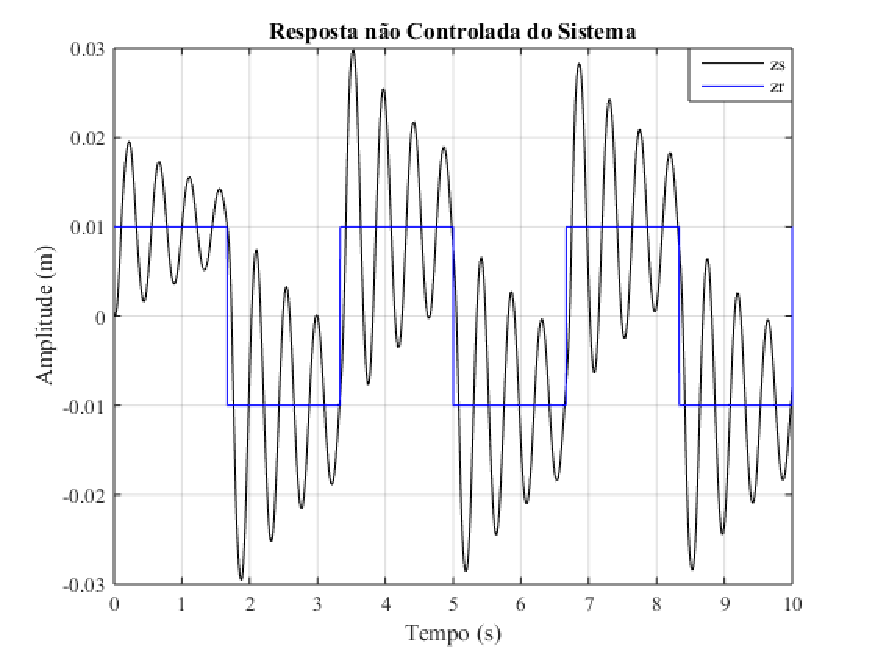
\includegraphics[width=.5\columnwidth]{./imagens/sistema_malha_fechada.pdf}
    \renewcommand{\figurename}{Fig. 2}
    \caption{Resposta do Sistema em Malha Fechada.}
  \label{mfechada}
\end{figure}
\end{frame}

\subsection{Projeto do Controlador}
\begin{frame}
\frametitle{Função de Transferência: Projeto do Controlador}
\begin{itemize}
\item A planta possui um atuador responsável por aplicar a força de controle $F_c$, o objetivo é encontrar a equação para o controlador, $G_c(s)$, de modo a minimizar as ondulações geradas pelo efeito da perturbação $z_r$. A Figura \ref{blocos} mostra a disposição dos blocos do sistema controlado.
\end{itemize}

\begin{figure}[H]
  \centering
  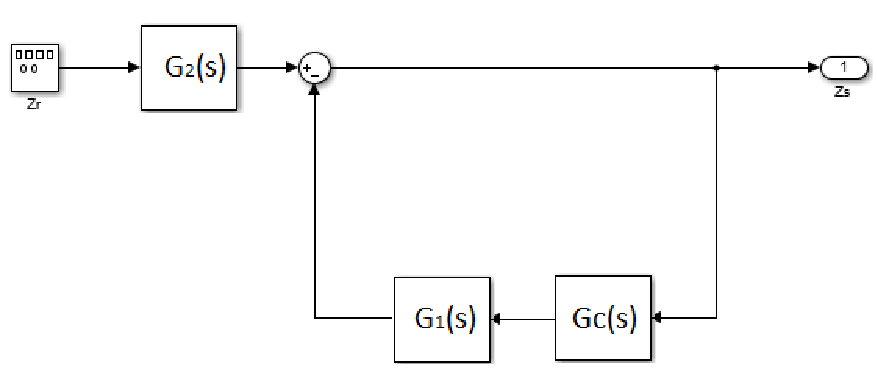
\includegraphics[width=.65\columnwidth]{./imagens/diagrama_malha_fechada.pdf}
    \renewcommand{\figurename}{Fig. 3}
    \caption{Diagrama de Blocos do Sistema controlado.}
  \label{blocos}
\end{figure}
\end{frame}

\begin{frame}
\frametitle{Função de Transferência: Projeto do Controlador}
\begin{itemize}
\item A Equação (\ref{essa}) traz a Função de Transferência do controlador a ser utilizado.
\end{itemize}

\begin{equation}\label{essa}
G_c(s)=\frac{A_{G_c}s^3+B_{G_c}s^2+C_{G_c}s+D_{G_c}}{E_{G_c}s+F_{G_c}}
\end{equation}

\begin{itemize}
\item Esse formato proporcionou a mesma quantidade de equações e de coeficientes de $G_c(s)$, condição necessária para que a alocação de polos seja realizada.
\end{itemize}
\end{frame}

\begin{frame}
\frametitle{Função de Transferência: Projeto do Controlador}
\begin{itemize}
\item A equação de malha fechada é representada pela Equação (\ref{eqmf}).
\end{itemize}

\begin{equation}\label{eqmf}
T(s) = G_2(s)\frac{1}{1+G_1(s)G_c(s)} 
\end{equation}
%\begin{itemize}
%\item Sendo $G_1(s)=\frac{nG_1(s)}{dG_1(s)}$ e $G_2(s)=\frac{nG_2(s)}{dG_2(s)}$, e $G_c(s)=\frac{nG_c(s)}{dG_c(s)}$.
%\end{itemize}

% \begin{itemize}
% \item Depois de efetuar uma simplificação, foi encontrada a Equação (\ref{oito}), que apresenta a função de transferência de malha fechada, $T(s)$.
% \end{itemize}
% \begin{equation}\label{oito}
% T(s)=\frac{nT(s)}{dT(s)}=\frac{nG_2(s)dG_c(s)}{dG(s)dG_c(s)+nG_1(s)nG_c(s)}
% \end{equation}
\end{frame}

% \begin{frame}
% \frametitle{Função de Transferência: Projeto do Controlador}
% \begin{itemize}
% \item A função $T(s)$ pode ser reescrita como mostram as Equações (\ref{seis}), (\ref{sete}) e (\ref{oito}).
% \end{itemize}
% \begin{equation}\label{seis}
% T(s) = \frac{nG_2(s)}{dG_2 (s)}\frac{1}{\frac{dG_1(s)dG_c(s)+nG_1(s)nG_c(s)}{dG_1(s)dG_c(s)}}
% \end{equation}

% \begin{itemize}
% \item Como $dG_1(s)$ e $dG_2(s)$ são iguais, podemos chamar ambos de $dG(s)$,
% \end{itemize}

% \begin{equation}\label{sete}
% T(s) = \frac{nG_2(s)dG(s)dG_c(s)}{dG(s)dG(s)dG_c(s)+dG(s)nG_1(s)nG_c(s)}
% \end{equation}

% \begin{itemize}
% \item Depois de efetuar uma simplificação, foi encontrada a Equação (\ref{oito}), que apresenta a função de transferência de malha fechada, $T(s)$.
% \end{itemize}

% \begin{equation}\label{oito}
% T(s)=\frac{nG_2(s)dG_c(s)}{dG(s)dG_c(s)+nG_1(s)nG_c(s)}
% \end{equation}
% \end{frame}

\begin{frame}
\frametitle{Função de Transferência: Projeto do Controlador}
\begin{itemize}
\item Para o projeto utilizando como controlador $G_c(s)$, os polos foram alocados com o intuito de eliminar o efeito dos zeros. Foram alocados polos em:
\begin{itemize}
\item $p_1 = -5$;
\item $p_2 = -120$;
\item $p_3 = -250$;
\item $p_{4,5} = -7,1720 \pm j28,6880$.
\end{itemize}
\item Conhecendo os polos, o denominador da função de transferência de malha fechada, $dT(s) = (s^2+2\xi \omega_n s+ \omega_n^2)(s+p_1)(s+p_2)(s+p_3)$, pode ser encontrado.
\end{itemize}
\end{frame}

% \begin{frame}
% \frametitle{Função de Transferência: Projeto do Controlador}
% \begin{itemize}
% \item Conhecendo os polos, o denominador da função de transferência de malha fechada, $dT(s) = (s^2+2\xi \omega_n s+ \omega_n^2)(s+p_1)(s+p_2)(s+p_3)$, pode ser encontrado. A Equação (\ref{dTs}) se refere a $dT(s)$.
% \end{itemize}

% \begin{equation}\label{dTs}
% \begin{matrix}
% dT(s)=s^5+389,344s^4+ 3,8103\times10^4s^3\\+9,3477\times10^5s^2+3,0002\times10^7s+1,3117\times10^8
% \end{matrix}
% \end{equation}
% \end{frame}

\begin{frame}
\frametitle{Função de Transferência: Projeto do Controlador}
\begin{itemize}
\item Conhecendo o denominador de malha fechada, foi possível encontrar os coeficientes do controlador, através da resolução de um sistema de equações lineares, no formato $Aw=b$.
\begin{itemize}
\item $A$: matriz composta pelos coeficientes da função de transferência da planta.
\item $b$: vetor composto pelos coeficientes de $dT(s)$.
\item $w$: vetor composto pelos coeficientes do controlador, a serem encontrados.
\end{itemize}
\end{itemize}
\end{frame}

% \begin{frame}
% \frametitle{Função de Transferência: Projeto do Controlador}
% \begin{equation}\label{matrizA}
% A = \begin{bmatrix}
%  1 & 0 & 0 & 0 & 2,45 & 0 \\ 
%  7,5 & 1 & 0 & 0 & 38,13 & 2,45 \\ 
%  1250 & 7,5 & 1 & 0 & 6205 & 38,13 \\ 
%  0 & 1250 & 7,5 & 1 & 13875 & 6205 \\
%  0 & 0 & 1250 & 7,5 & 1,125\times10^6 & 13875 \\
%  0 & 0 & 0 & 1250 & 0 & 1,125\times10^6
% \end{bmatrix}
% \end{equation}
% \end{frame}

% \begin{frame}
% \frametitle{Função de Transferência: Projeto do Controlador}
% \begin{equation}\label{vetorb}
% b = \begin{bmatrix}
%  1 \\ 
%  389,344 \\ 
%  3,8103\times10^4 \\ 
%  9,3477\times10^5 \\
%  3,0002\times10^7 \\
%  1,3117\times10^8
% \end{bmatrix}
% \end{equation}

% \begin{equation}\label{gcs}
% G_c(s) = \frac{-9,531 s^3 + 15,42 s^2 + 1,885\times10^4 s + 1520}{4,298 s + 114,9}
% \end{equation}
% \end{frame}

\section{Projeto usando Espaço de Estados (EE)}
\begin{frame}
\Huge{\centerline{Projeto usando}}
\Huge{\centerline{Espaço de Estados}}
\end{frame}
\subsection{Modelagem do Sistema}
\begin{frame}
\frametitle{Espaço de Estados: Modelagem do Sistema}
\begin{itemize}
\item Para o Sistema de Suspensão Ativa, foram definidos como vetor de estados, $x$, vetor de entrada, $u$, e vetor de saída, $y$, os apresentados nas Equações (\ref{vetorx}), (\ref{vetoru}), (\ref{vetory}) \cite{quanser}.
\end{itemize}
\begin{equation}\label{vetorx}
x=\left[ \begin{matrix}
z_s-z_{us} \\
\dot{z_s} \\
z_{us}-z_r \\
\dot{z_{us}}
\end{matrix} \right]
\end{equation}

\begin{equation}\label{vetoru}
u=\left[\begin{matrix}
\dot{z_r} \\
F_c
\end{matrix}\right]
\end{equation}

\begin{equation}\label{vetory}
y=\left[\begin{matrix}
z_s-z_{us} \\
\ddot{z_s} \\
\end{matrix}\right]
\end{equation}
\end{frame}

\begin{frame}
\frametitle{Espaço de Estados: Modelagem do Sistema}
\begin{itemize}
\item Através das equações diferenciais que representam o sistema, foi possível calcular as matrizes $A$, $B$, $C$ e $D$. As Equações (\ref{matriza}), (\ref{matrizb}), (\ref{matrizc}), e (\ref{matrizd}) trazem essas matrizes.
\end{itemize}
\begin{equation}\label{matriza}
A=\left[\begin{matrix}
0 & 1 & 0 & -1 \\
-\frac{K_s}{M_s} & -\frac{B_s}{M_s} & 0 & \frac{B_s}{M_s} \\
0 & 0 & 0 & 1 \\
\frac{K_s}{M_{us}} & \frac{B_s}{M_{us}} & -\frac{K_{us}}{M_{us}} & -\frac{B_s+B_{us}}{M_{us}}
\end{matrix} \right]
\end{equation}

\begin{equation}\label{matrizb}
B=\left[\begin{matrix}
0 & 0 \\
0 & \frac{1}{M_s} \\
-1 & 0 \\
\frac{B_{us}}{M_{us}} & -\frac{1}{M_{us}}
\end{matrix}\right]
\end{equation}
\end{frame}

\begin{frame}
\frametitle{Espaço de Estados: Modelagem do Sistema}
\begin{equation}\label{matrizc}
C=\left[\begin{matrix}
1 & 0 & 0 & 0 \\
-\frac{K_s}{M_s} & -\frac{B_s}{M_s} & 0 & \frac{B_s}{M_s}
\end{matrix}\right]
\end{equation}

\begin{equation}\label{matrizd}
D=\left[ \begin{matrix}
0 & 0 \\
0 & \frac{1}{M_s}
\end{matrix} \right]
\end{equation}
\end{frame}

\begin{frame}
\frametitle{Espaço de Estados: Modelagem do Sistema}
\begin{itemize}
\item Na Figura \ref{modeloSimulink2} é apresentado o diagrama de blocos do sistema.
\end{itemize}
\begin{figure}[H]
	\centering
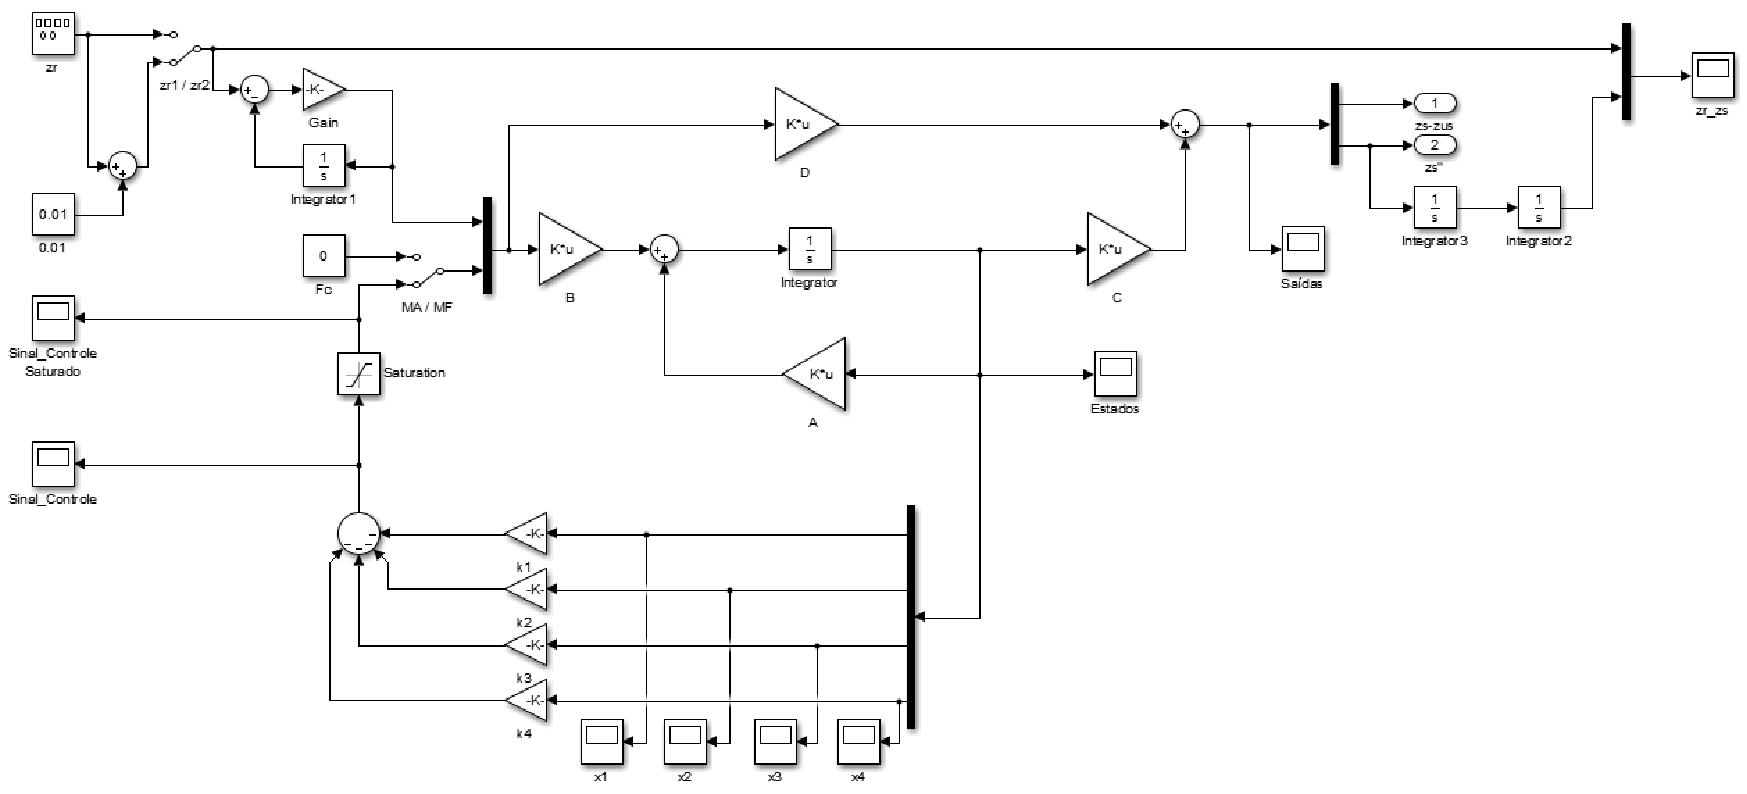
\includegraphics[width=\columnwidth]{./imagens/modeloSimulink_malha_fechada.pdf}
    \renewcommand{\figurename}{Fig. 4}
    \caption{Diagrama de Blocos do Sistema de Suspensão Ativa.}
	\label{modeloSimulink2}
\end{figure}
\end{frame}

\begin{frame}
\frametitle{Espaço de Estados: Modelagem do Sistema}
\begin{itemize}
\item A Figura \ref{malhaabertaEE} apresenta a resposta natural do sistema, considerando $z_r$ variando de $-0,01$ à $0,01$m.
\end{itemize}
\begin{figure}[H]
	\centering
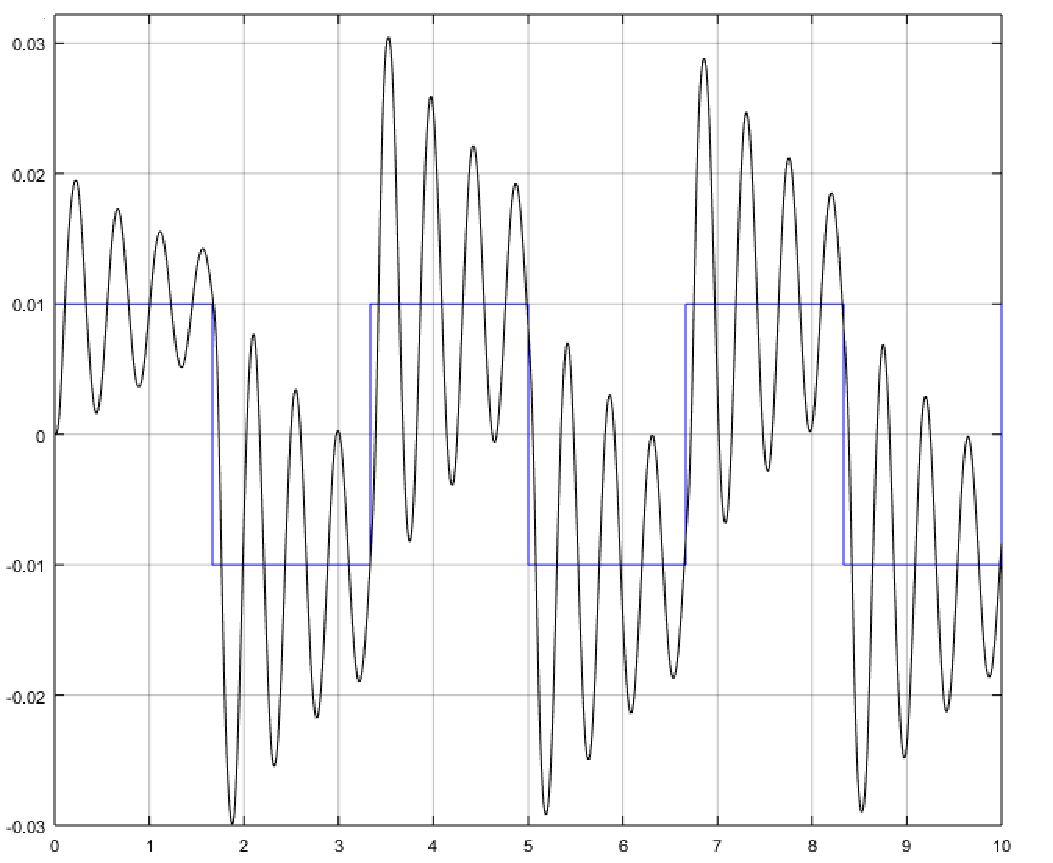
\includegraphics[width=.55\columnwidth]{./imagens/resposta_natural_sistema.pdf}
	\renewcommand{\figurename}{Fig. 5}
    \caption{Resposta Natural do Sistema, $z_r$ de $-0,01$ à $0,01$m.}
	\label{malhaabertaEE}
\end{figure}
\end{frame}

\begin{frame}
\frametitle{Espaço de Estados: Modelagem do Sistema}
\begin{itemize}
\item A Figura \ref{malhaabertaEE2} apresenta a resposta natural do sistema, considerando $z_r$ variando de $0$ à $0,02$m.
\end{itemize}
\begin{figure}[H]
	\centering
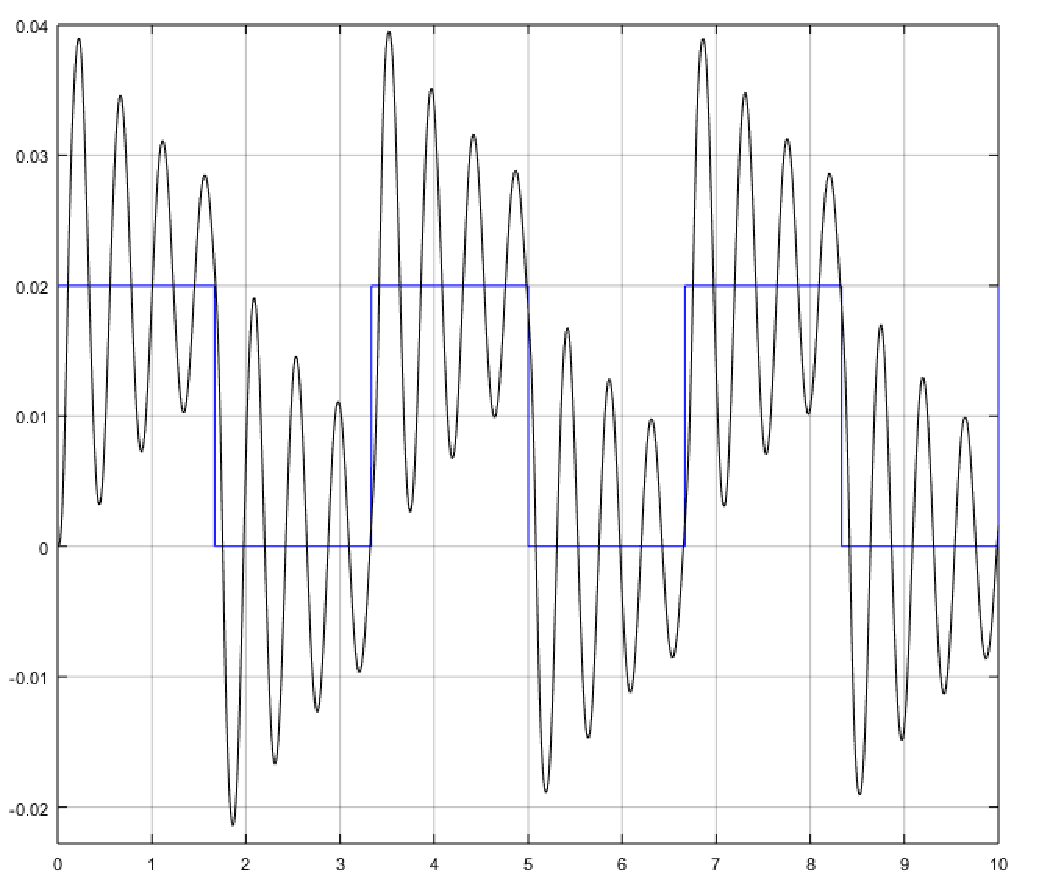
\includegraphics[width=.55\columnwidth]{./imagens/resposta_natural_sistema2.pdf}
    \renewcommand{\figurename}{Fig. 6}
    \caption{Resposta Natural do Sistema, $z_r$ de $0$ à $0,02$m.}
	\label{malhaabertaEE2}
\end{figure}
\end{frame}

\subsection{Projeto do Controlador}
\begin{frame}
\frametitle{Espaço de Estados: Projeto do Controlador}
\begin{itemize}
\item Através das funções \textit{ctrb} e \textit{obsv} do \textit{matlab} foram verificadas a controlabilidade e a observabilidade do sistema, respectivamente.
\item Com a utlização da função \textit{eig} do \textit{matlab} foi possível conhecer os autovalores da matriz $A$, ou seja, os polos do sistema.
\item Dois pares de polos complexos em: $p_{1,2}= -0,6087 \pm j14,0644$ e $p_{3,4}=-7,1719 \pm j47,5981$.

\item Especificações do projeto
\begin{itemize}
\item Sobrelevação máxima, $M_p$, de $5\%$, e o tempo de estabelecimento, $t_s$, de $0,5$ segundos.
\item Par de polos dominantes em $p_{1,2} = -8 \pm j8,3895$.
\item O outro par de polos foi escolhido em $p_{3,4} = -9,9596 \pm j35,2870$.
\end{itemize}
\end{itemize}
\end{frame}

\begin{frame}
\frametitle{Espaço de Estados: Projeto do Controlador}
\begin{itemize}
\item Para encontrar a matriz de ganho $K$ através da fórmula de Ackermann, foi utilizada a função \textit{acker} do \textit{matlab}.
\item A Equação (\ref{matrizk}) apresenta a matriz $K$ encontrada no projeto.
\end{itemize}

\begin{equation}\label{matrizk}
K = \left[ \begin{matrix}
-545,9043 & 38,4895 & 45,0246 & -4,6480
\end{matrix} \right]
\end{equation}
\end{frame}

\section{Resultados}
\begin{frame}
\Huge{\centerline{Resultados:}}
\Huge{\centerline{Projeto usando FT}}
\end{frame}
\subsection{Projeto usando Função de Transferência}
\begin{frame}
\frametitle{Função de Transferência: Resultados}
\begin{itemize}
\item A Figura \ref{mfechadacontrolada} mostra a resposta do sistema com a ação do controlador.
\end{itemize}
\begin{figure}[H]
	\centering
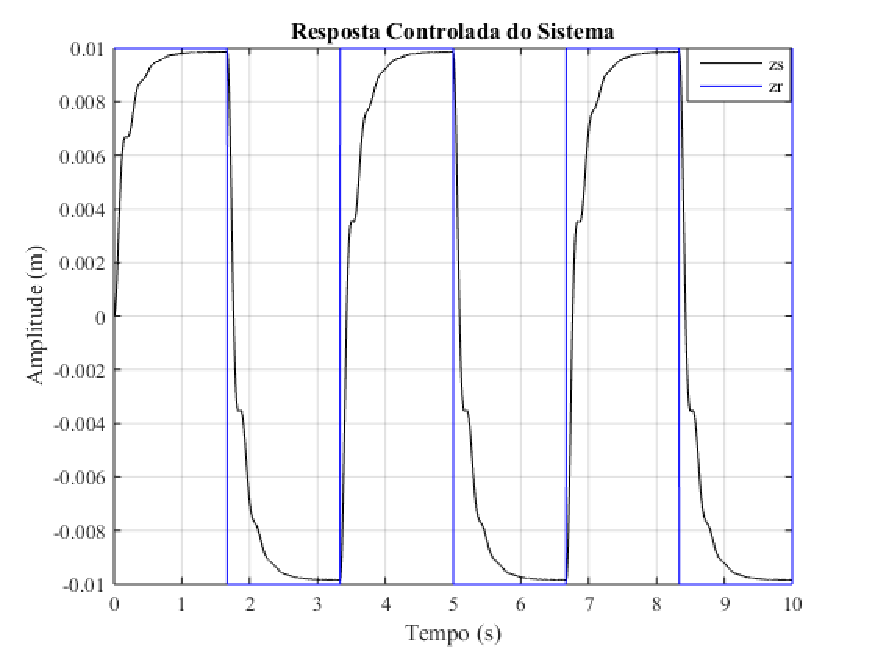
\includegraphics[width=.5\columnwidth]{./imagens/resposta_controlada.pdf}
    \renewcommand{\figurename}{Fig. 7}
    \caption{Resposta do Sistema com Controlador.}
	\label{mfechadacontrolada}
\end{figure}
\end{frame}

\begin{frame}
\frametitle{Função de Transferência: Resultados}
\begin{itemize}
\item A Figura \ref{sinalcontrole} apresenta o Sinal de Controle resultante da ação de $G_c(s)$.
\end{itemize}
\begin{figure}[H]
	\centering
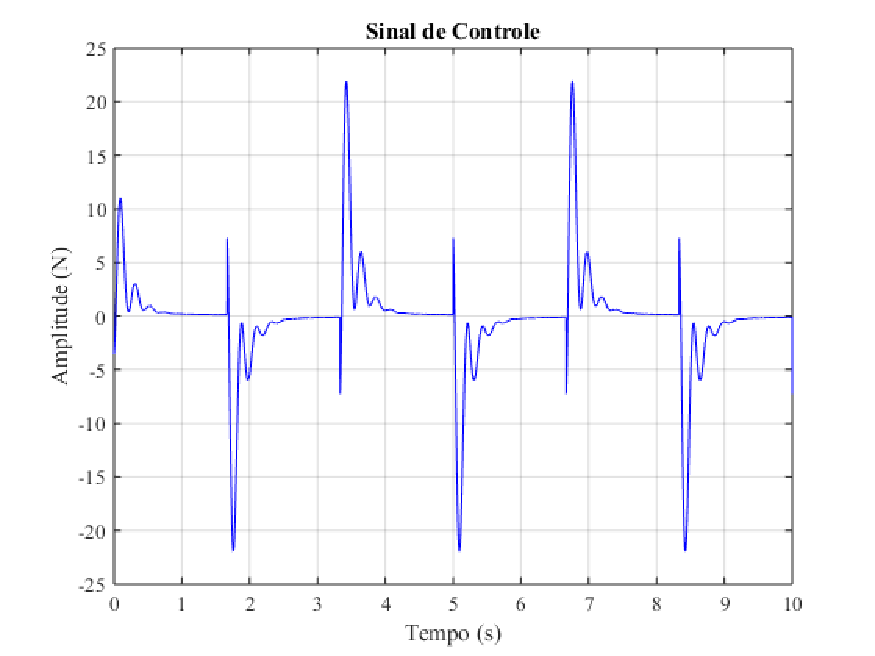
\includegraphics[width=.5\columnwidth]{./imagens/sinal_de_controle.pdf}
    \renewcommand{\figurename}{Fig. 8}
    \caption{Sinal de Controle do Sistema.}
	\label{sinalcontrole}
\end{figure}
\end{frame}

\subsubsection{Teste de Robustez do Controlador $G_c(s)$}
\begin{frame}
\frametitle{Função de Transferência: Resultados}
\framesubtitle{Teste de Robustez do Controlador $G_c(s)$}
\begin{itemize}
\item No primeiro caso foram levadas em consideração as variações de $K_s$ e $K_{us}$ em 3\%, e de $B_s$ e $B_{us}$ em 10\%.
\item Para as simulações, foram utilizados 7 valores do intervalo de cada parâmetro que sofreu variação, totalizando 2401 iterações.
\end{itemize}
\end{frame}

\begin{frame}
\frametitle{Função de Transferência: Resultados}
\framesubtitle{Teste de Robustez do Controlador $G_c(s)$}
\begin{itemize}
\item A Figura \ref{sistemaIntervalar} traz as várias respostas do Sistema, sem a presença do controlador, com variação dos parâmetros, em Malha Fechada.
\end{itemize}
\begin{figure}[H]
	\centering
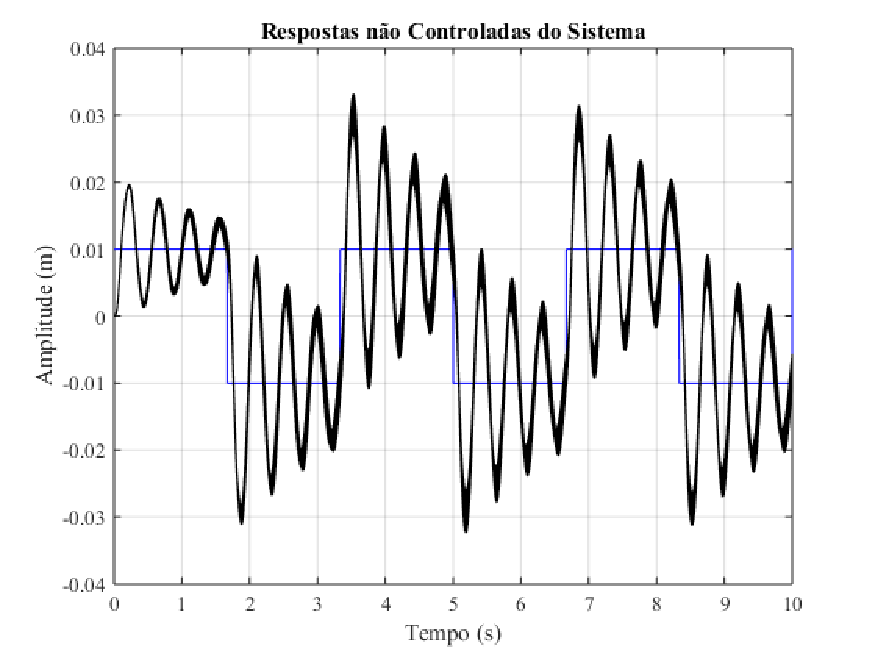
\includegraphics[width=.5\columnwidth]{./imagens/resposta_sistema_variando_Ks_Kus_Bs_Bus.pdf}
    \renewcommand{\figurename}{Fig. 9}
    \caption{Respostas não Controladas do Sistema com variação de $K_s$ e $K_{us}$ em 3\%, e $B_s$ e $B_{us}$ em 10\%.}
	\label{sistemaIntervalar}
\end{figure}
\end{frame}

\begin{frame}
\frametitle{Função de Transferência: Resultados}
\framesubtitle{Teste de Robustez do Controlador $G_c(s)$}
\begin{itemize}
\item A Figura \ref{controladaIntervalar} apresenta as respostas do Sistema, com a ação do controlador $G_c(s)$.
\end{itemize}
\begin{figure}[H]
	\centering
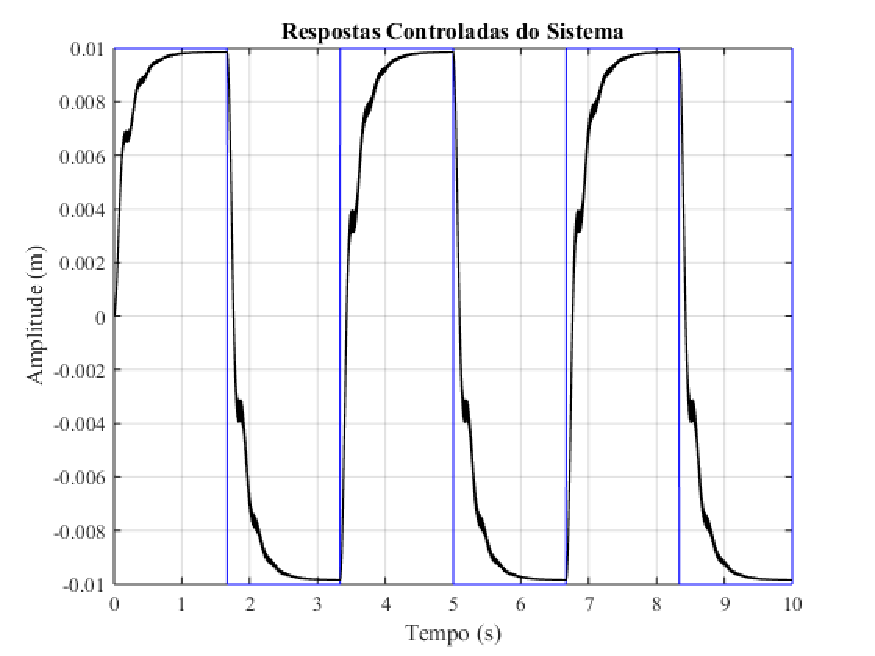
\includegraphics[width=.5\columnwidth]{./imagens/resposta_controlada_variando_Ks_Kus_Bs_Bus_controlador_sem_robustez.pdf}
    \renewcommand{\figurename}{Fig. 10}
    \caption{Respostas Controladas do Sistema com variação de $K_s$ e $K_{us}$ em 3\%, e $B_s$ e $B_{us}$ em 10\%.}
	\label{controladaIntervalar}
\end{figure}
\end{frame}

\begin{frame}
\frametitle{Função de Transferência: Resultados}
\framesubtitle{Teste de Robustez do Controlador $G_c(s)$}
\begin{itemize}
\item A Figura \ref{sinalcontroleIntervalar} mostra os vários Sinais de Controle resultantes da ação de $G_c(s)$ e a variação de parâmetros da planta.
\end{itemize}
\begin{figure}[H]
  \centering
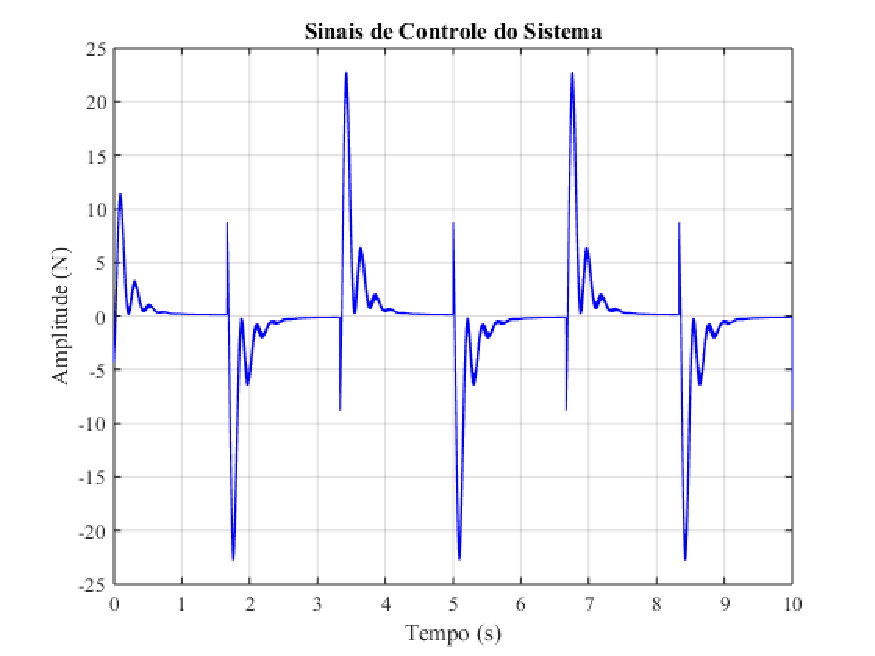
\includegraphics[width=.5\columnwidth]{./imagens/sinal_de_controle_variando_Ks_Kus_Bs_Bus_controlador_sem_robustez.pdf}
  \renewcommand{\figurename}{Fig. 11}
    \caption{Sinais de Controle do Sistema com variação de $K_s$ e $K_{us}$ em 3\%, e $B_s$ e $B_{us}$ em 10\%.}
  \label{sinalcontroleIntervalar}
\end{figure}
\end{frame}

\begin{frame}
\frametitle{Função de Transferência: Resultados}
\framesubtitle{Teste de Robustez do Controlador $G_c(s)$}
\begin{itemize}
\item No segundo caso foram levadas em consideração as variações de $K_s$ e $K_{us}$ em 5\%, e de $B_s$ e $B_{us}$ em 10\%.
\item Para as simulações, foram utilizados 7 valores do intervalo de cada parâmetro que sofreu variação, totalizando 2401 iterações.
\end{itemize}
\end{frame}

\begin{frame}
\frametitle{Função de Transferência: Resultados}
\framesubtitle{Teste de Robustez do Controlador $G_c(s)$}
\begin{itemize}
\item A Figura \ref{sistemaIntervalar2} traz as várias respostas do Sistema, sem a presença do controlador, com variação dos parâmetros, em Malha Fechada.
\end{itemize}
\begin{figure}[H]
  \centering
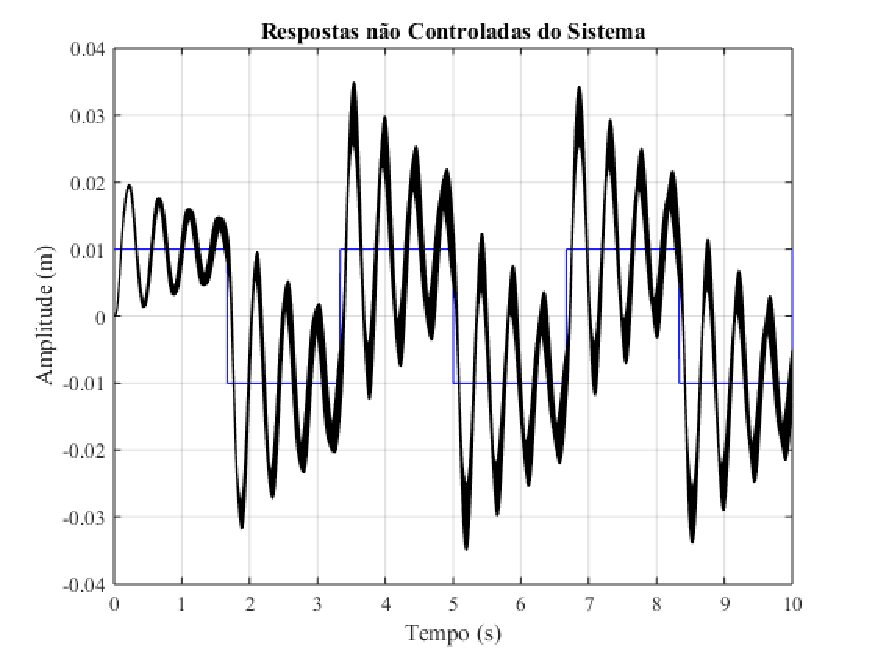
\includegraphics[width=.5\columnwidth]{./imagens/resposta_sistema_variando_Ks_Kus_5_Bs_Bus_10.pdf}
    \renewcommand{\figurename}{Fig. 12}
    \caption{Respostas não Controladas do Sistema com variação de $K_s$ e $K_{us}$ em 5\%, e $B_s$ e $B_{us}$ em 10\%.}
  \label{sistemaIntervalar2}
\end{figure}
\end{frame}

\begin{frame}
\frametitle{Função de Transferência: Resultados}
\framesubtitle{Teste de Robustez do Controlador $G_c(s)$}
\begin{itemize}
\item A Figura \ref{controladaIntervalar2} apresenta as respostas do Sistema, com a ação do controlador $G_c(s)$.
\end{itemize}
\begin{figure}[H]
  \centering
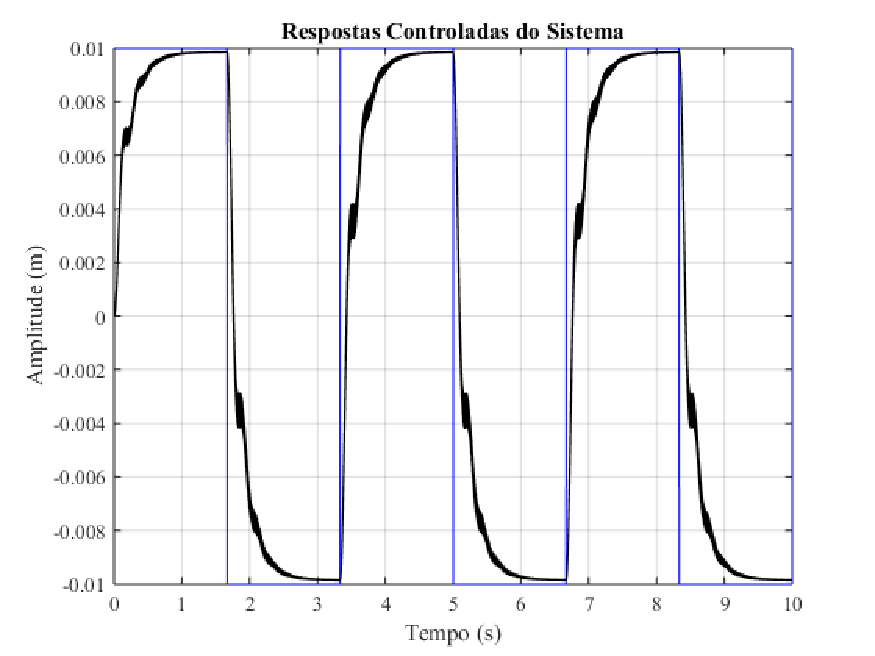
\includegraphics[width=.5\columnwidth]{./imagens/resposta_controlada_variando_Ks_Kus_5_Bs_Bus_10_controlador_sem_robustez.pdf}
    \renewcommand{\figurename}{Fig. 13}
    \caption{Respostas Controladas do Sistema com variação de $K_s$ e $K_{us}$ em 5\%, e $B_s$ e $B_{us}$ em 10\%.}
  \label{controladaIntervalar2}
\end{figure}
\end{frame}

\begin{frame}
\frametitle{Função de Transferência: Resultados}
\framesubtitle{Teste de Robustez do Controlador $G_c(s)$}
\begin{itemize}
\item A Figura \ref{sinalcontroleIntervalar2} mostra os vários Sinais de Controle resultantes da ação de $G_c(s)$ e a variação de parâmetros da planta.
\end{itemize}
\begin{figure}[H]
  \centering
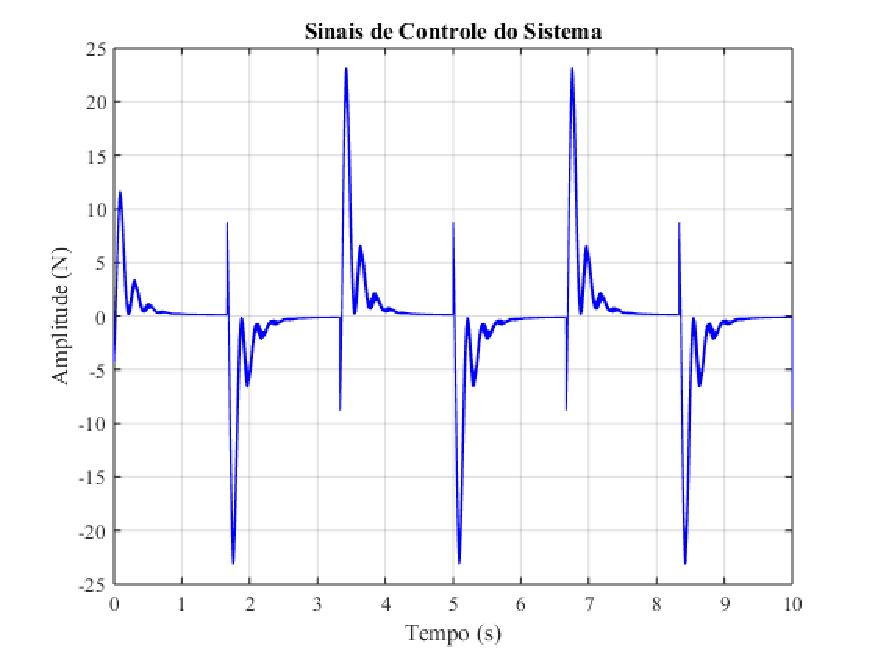
\includegraphics[width=.5\columnwidth]{./imagens/sinal_de_controle_variando_Ks_Kus_5_Bs_Bus_10_controlador_sem_robustez.pdf}
    \renewcommand{\figurename}{Fig. 14}
    \caption{Sinais de Controle do Sistema com variação de $K_s$ e $K_{us}$ em 5\%, e $B_s$ e $B_{us}$ em 10\%.}
  \label{sinalcontroleIntervalar2}
\end{figure}
\end{frame}

\subsection{Projeto usando Espaço de Estados}
\begin{frame}
\Huge{\centerline{Resultados:}}
\Huge{\centerline{Projeto usando EE}}
\end{frame}

\begin{frame}
\frametitle{Espaço de Estados: Resultados}
\begin{itemize}
\item A Figura \ref{malhafechadaEE} apresenta a resposta controlada do sistema, considerando $z_r$ de $-0,01$ a $0,01$m.
\end{itemize}
\begin{figure}[H]
	\centering
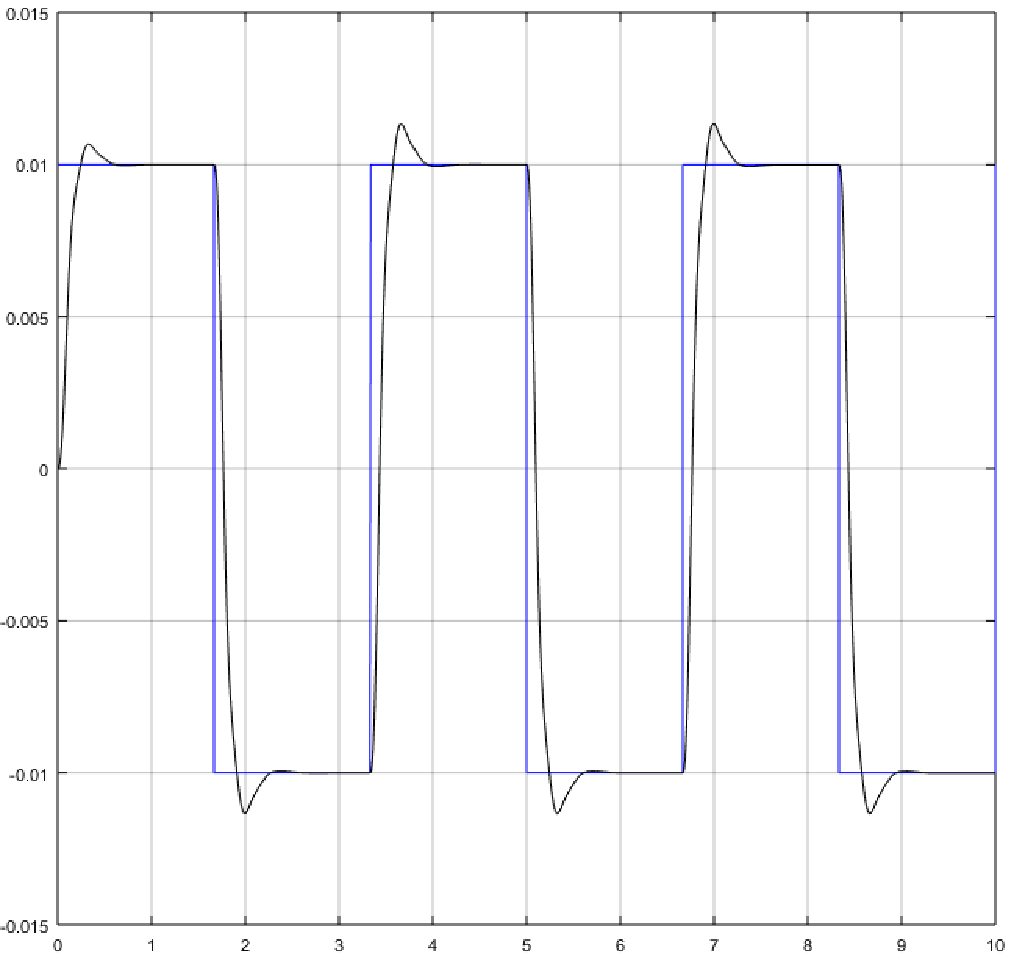
\includegraphics[width=.45\columnwidth]{./imagens/resposta_controlada_sistema.pdf}
    \renewcommand{\figurename}{Fig. 15}
    \caption{Resposta Controlada do Sistema, $z_r$ de $-0,01$ à $0,01$m.}
	\label{malhafechadaEE}
\end{figure}
\end{frame}

\begin{frame}
\frametitle{Espaço de Estados: Resultados}
\begin{itemize}
\item A Figura \ref{sinalcontroleEE} mostra o esforço de controle para alocar os polos nas posições desejadas, considerando $z_r$ de $-0,01$ a $0,01$m.
\end{itemize}
\begin{figure}[H]
	\centering
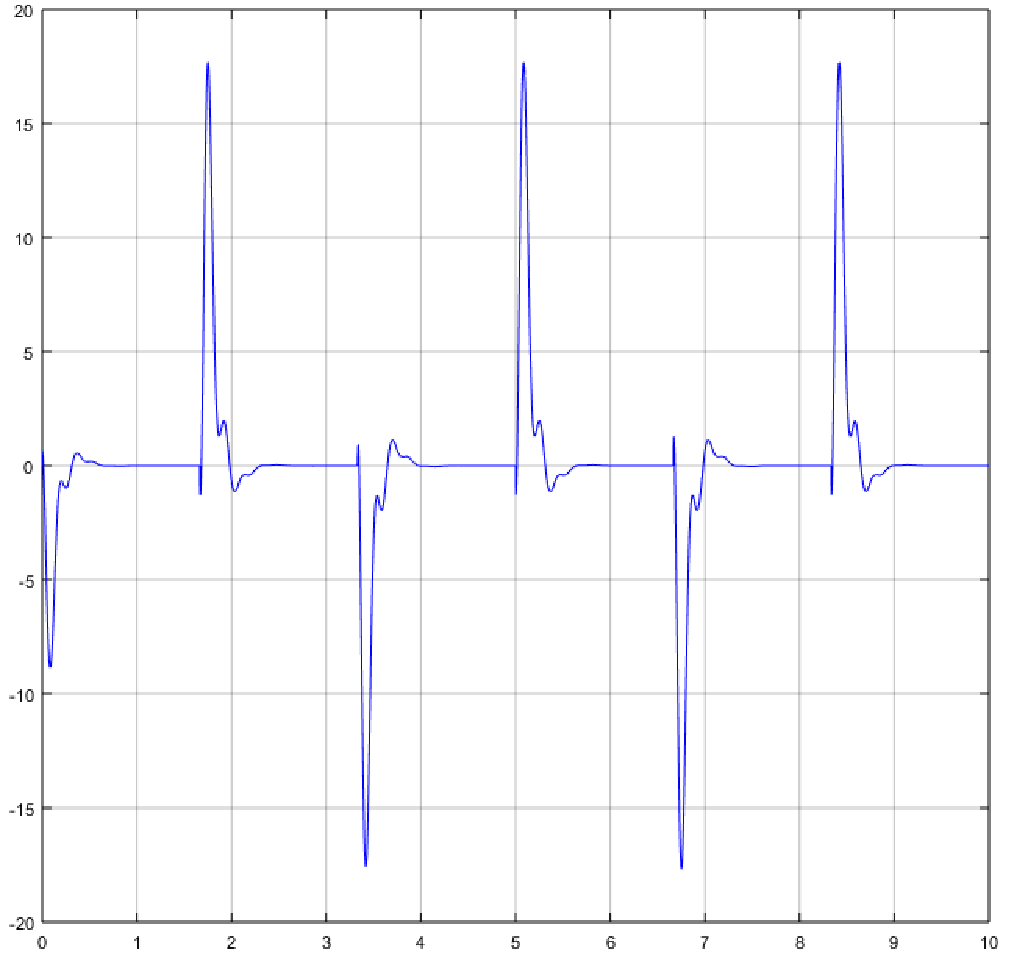
\includegraphics[width=.45\columnwidth]{./imagens/sinal_controle_sistema.pdf}
    \renewcommand{\figurename}{Fig. 16}
    \caption{Sinal de Controle do Sistema, $z_r$ de $-0,01$ à $0,01$m.}
	\label{sinalcontroleEE}
\end{figure}
\end{frame}

\begin{frame}
\frametitle{Espaço de Estados: Resultados}
\begin{itemize}
\item A Figura \ref{malhafechadaEE2} apresenta a resposta controlada do sistema, considerando $z_r$ de $0$ a $0,02$m.
\end{itemize}
\begin{figure}[H]
	\centering
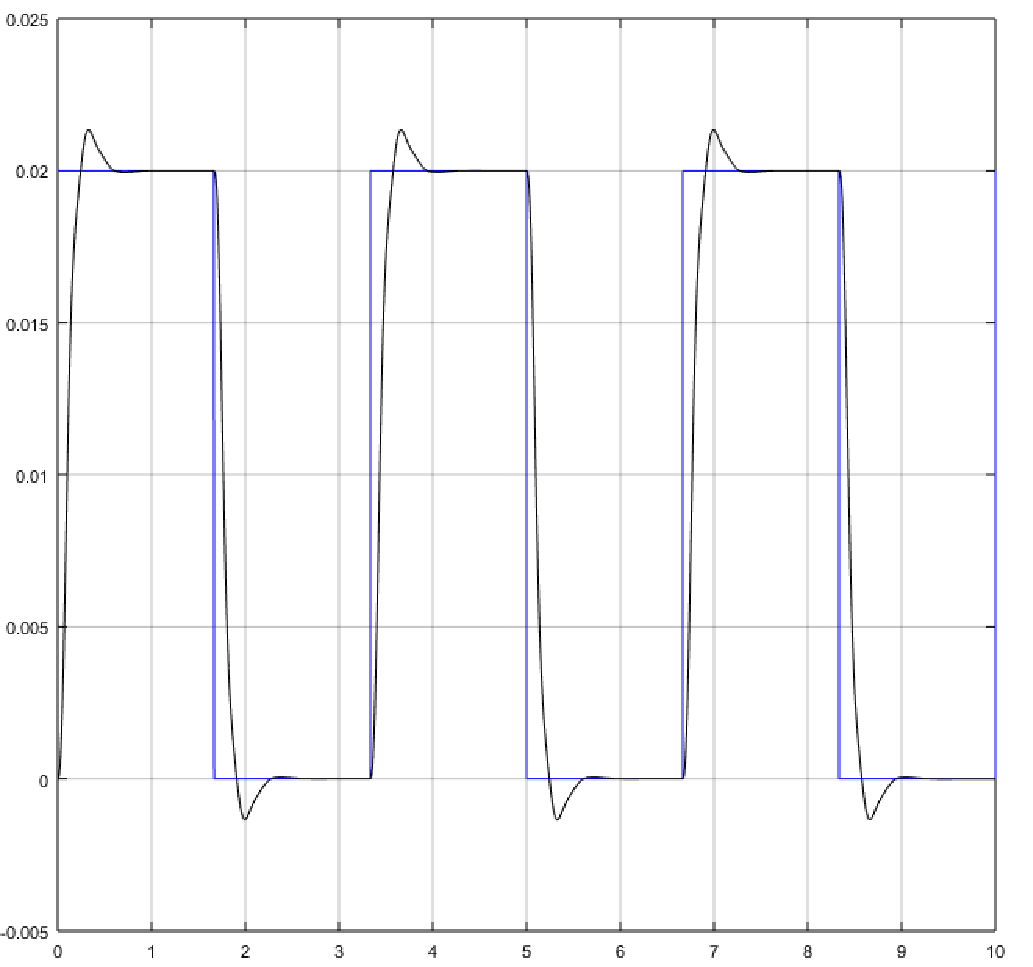
\includegraphics[width=.45\columnwidth]{./imagens/resposta_controlada_sistema2.pdf}
    \renewcommand{\figurename}{Fig. 17}
    \caption{Resposta Controlada do Sistema, $z_r$ de $0$ à $0,02$m.}
	\label{malhafechadaEE2}
\end{figure}
\end{frame}

\begin{frame}
\frametitle{Espaço de Estados: Resultados}
\begin{itemize}
\item A Figura \ref{sinalcontroleEE2} mostra o esforço de controle para alocar os polos nas posições desejadas, considerando $z_r$ de $0$ a $0,02$m.
\end{itemize}
\begin{figure}[H]
	\centering
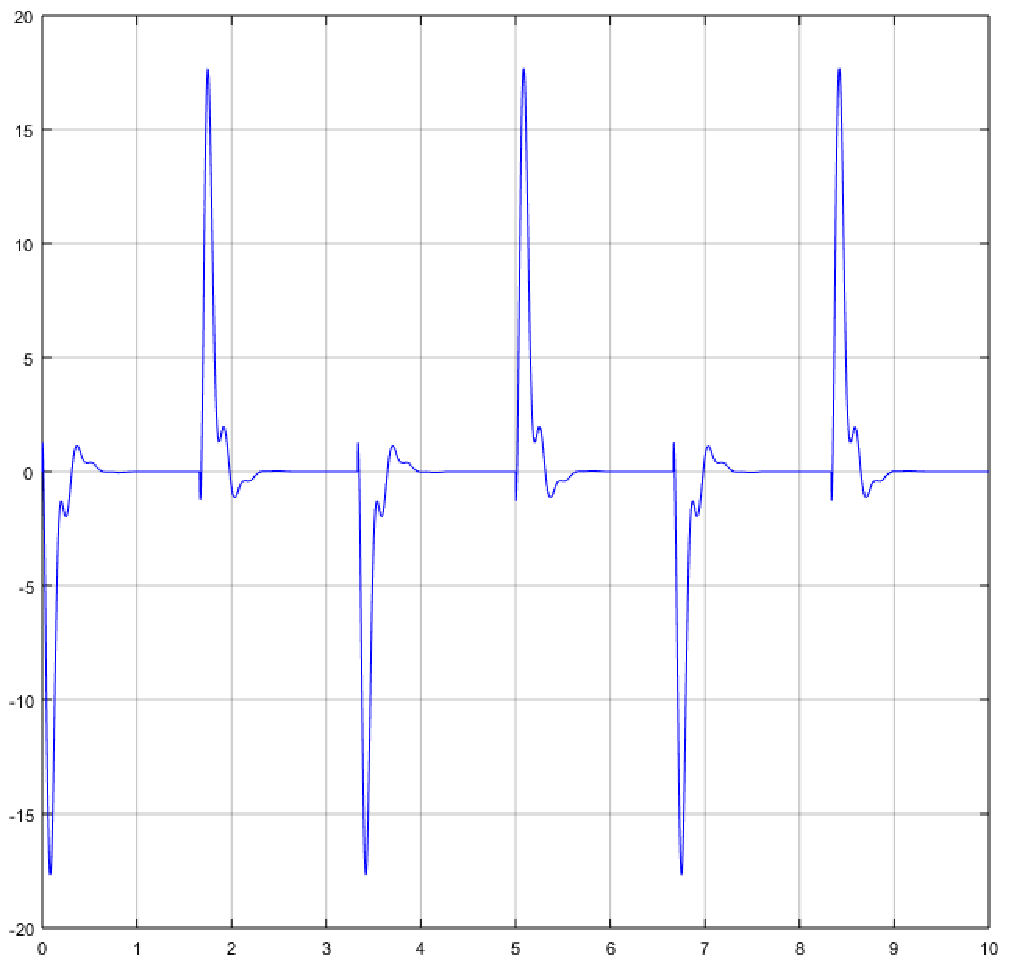
\includegraphics[width=.45\columnwidth]{./imagens/sinal_controle_sistema2.pdf}
    \renewcommand{\figurename}{Fig. 18}
    \caption{Sinal de Controle do Sistema, $z_r$ de $0$ à $0,02$m.}
	\label{sinalcontroleEE2}
\end{figure}
\end{frame}

\subsubsection{Projeto do Guia de Laboratório do Sistema de Suspensão Ativa da \protect\textit{Quanser}}
\begin{frame}
\frametitle{Espaço de Estados: Resultados}
\framesubtitle{Projeto do Guia de Laboratório do Sistema de Suspensão Ativa da \protect\textit{Quanser}}
\begin{itemize}
\item Na Guia de Laboratório do Sistema de Suspensão Ativa, fornecido pela \textit{Quanser}, há o projeto de um controlador por realimentação de estados. Nesse projeto é encontrada uma matriz de ganho $K = \left[\begin{matrix}
24,66 & 48,87 & -0,47 & 3,68 \end{matrix}\right]$ \cite{quanser}.
\end{itemize}
\end{frame}

\begin{frame}
\frametitle{Espaço de Estados: Resultados}
\framesubtitle{Projeto do Guia de Laboratório do Sistema de Suspensão Ativa da \protect\textit{Quanser}}
\begin{itemize}
\item A Figura \ref{quanserE} apresenta a resposta controlada do sistema, considerando $z_r$ de $-0,01$ à $0,01$m.
\end{itemize}
\begin{figure}[H]
	\centering
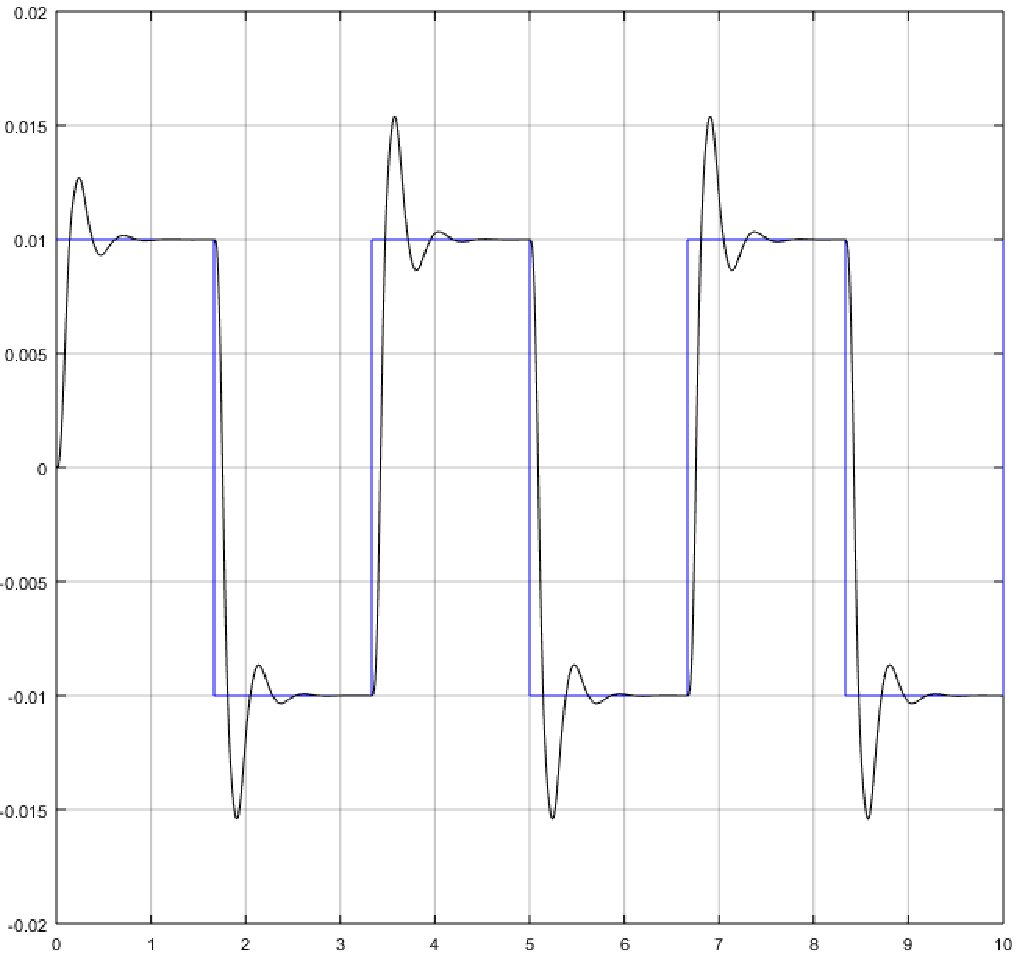
\includegraphics[width=.45\columnwidth]{./imagens/quanserE.pdf}
    \renewcommand{\figurename}{Fig. 19}
    \caption{Resposta Controlada do Sistema, $z_r$ de $-0,01$ à $0,01$m.}
	\label{quanserE}
\end{figure}
\end{frame}

\begin{frame}
\frametitle{Espaço de Estados: Resultados}
\framesubtitle{Projeto do Guia de Laboratório do Sistema de Suspensão Ativa da \protect\textit{Quanser}}
\begin{itemize}
\item A Figura \ref{quanserE2} mostra o esforço de controle do sistema, considerando $z_r$ de $-0,01$ à $0,01$m.
\end{itemize}
\begin{figure}[H]
	\centering
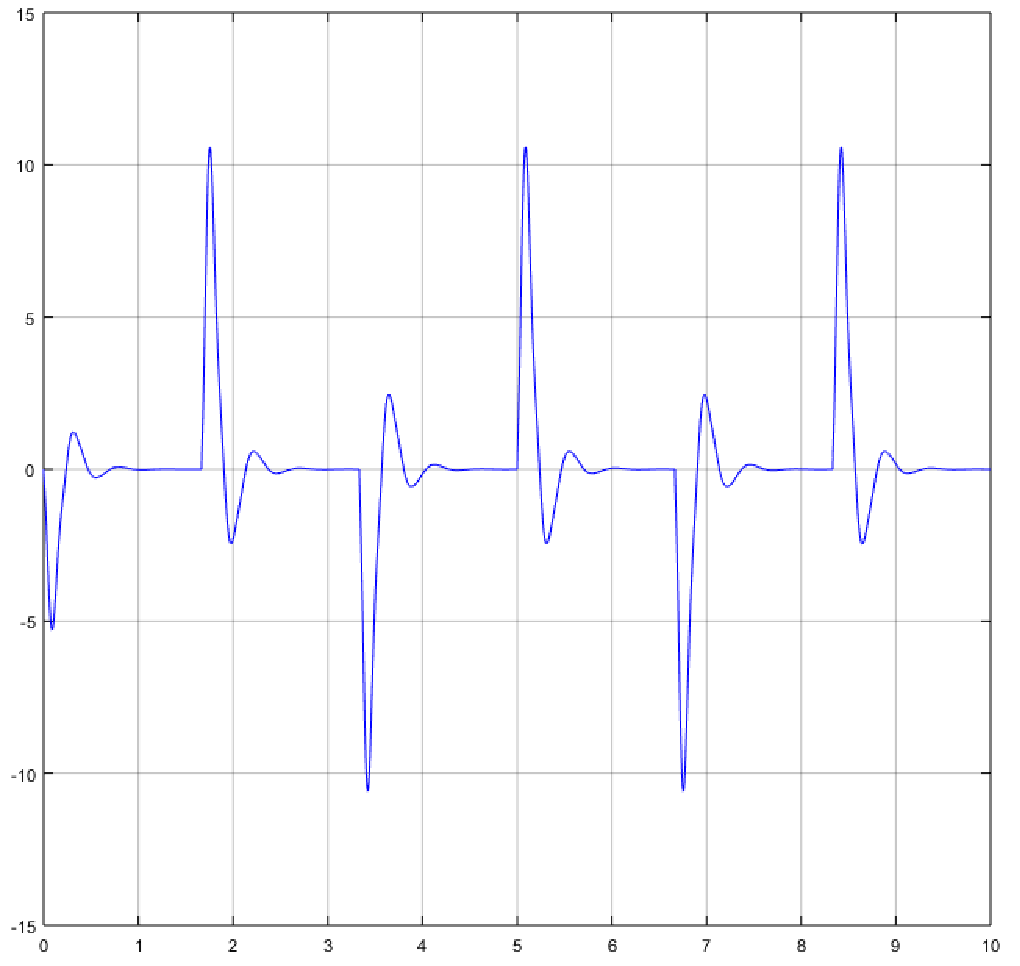
\includegraphics[width=.45\columnwidth]{./imagens/quanserE2.pdf}
    \renewcommand{\figurename}{Fig. 20}
    \caption{Sinal de Controle do Sistema, $z_r$ de $-0,01$ à $0,01$m.}
	\label{quanserE2}
\end{figure}
\end{frame}

\begin{frame}
\frametitle{Espaço de Estados: Resultados}
\framesubtitle{Projeto do Guia de Laboratório do Sistema de Suspensão Ativa da \protect\textit{Quanser}}
\begin{itemize}
\item A Figura \ref{quanserEE} apresenta a resposta controlada do sistema, considerando $z_r$ de $0$ à $0,02$m.
\end{itemize}
\begin{figure}[H]
	\centering
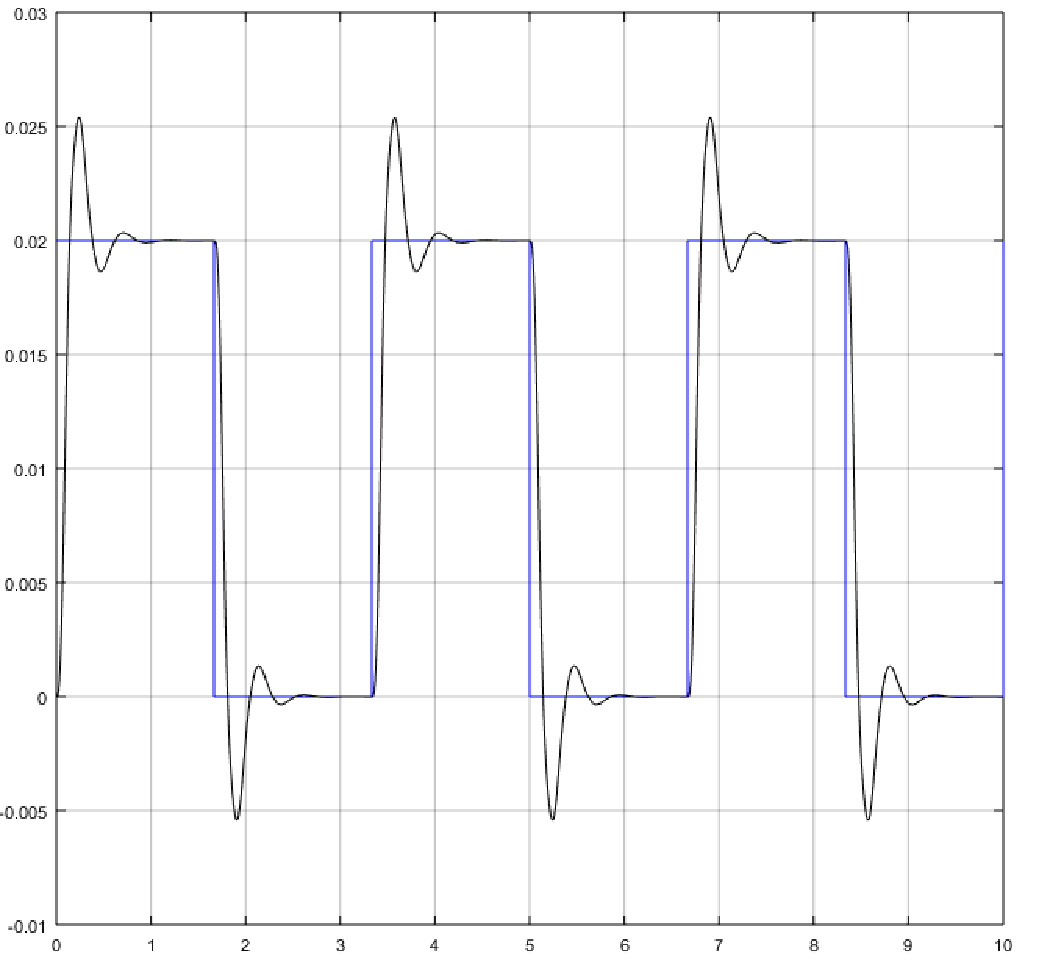
\includegraphics[width=.45\columnwidth]{./imagens/quanserEE.pdf}
    \renewcommand{\figurename}{Fig. 21}
    \caption{Resposta Controlada do Sistema, $z_r$ de $0$ à $0,02$m.}
	\label{quanserEE}
\end{figure}
\end{frame}

\begin{frame}
\frametitle{Espaço de Estados: Resultados}
\framesubtitle{Projeto do Guia de Laboratório do Sistema de Suspensão Ativa da \protect\textit{Quanser}}
\begin{itemize}
\item A Figura \ref{quanserEE2} mostra o esforço de controle do sistema, considerando $z_r$ de $0$ à $0,02$m.
\end{itemize}
\begin{figure}[H]
	\centering
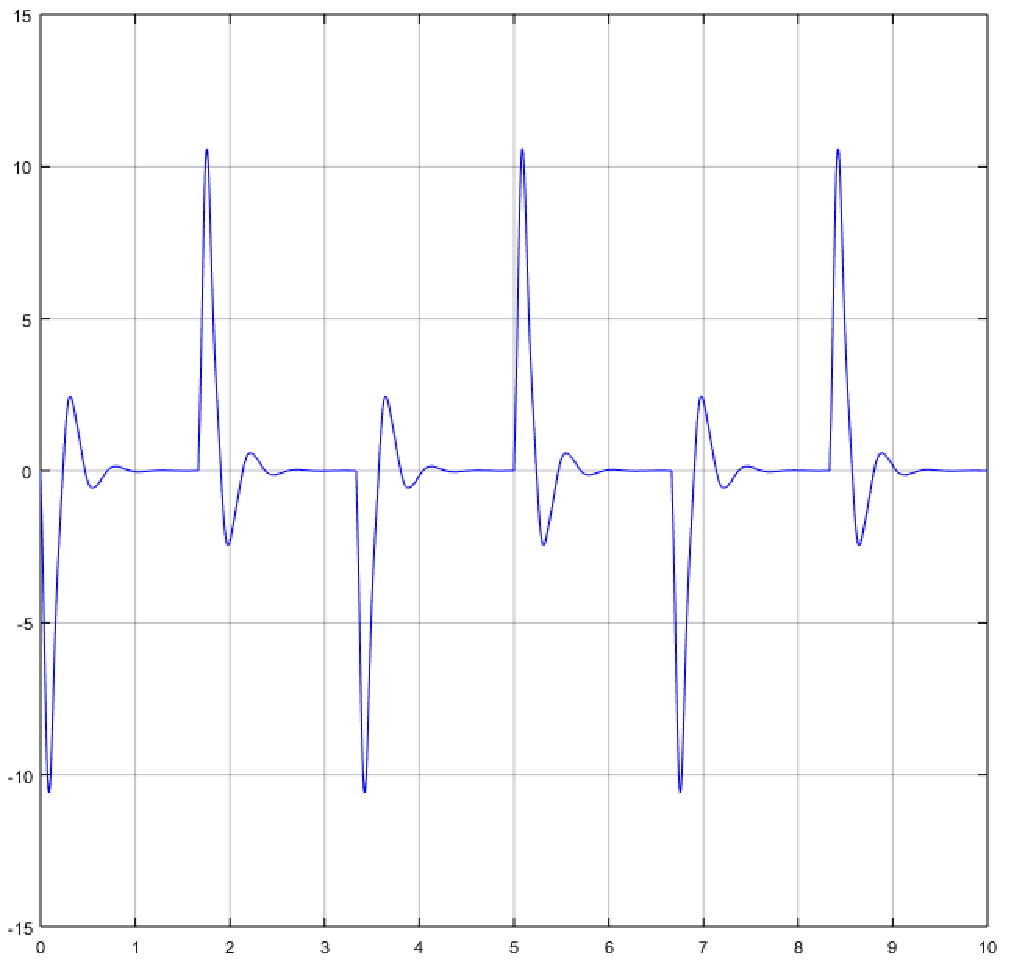
\includegraphics[width=.45\columnwidth]{./imagens/quanserEE2.pdf}
    \renewcommand{\figurename}{Fig. 22}
    \caption{Sinal de Controle do Sistema, $z_r$ de $0$ à $0,02$m.}
	\label{quanserEE2}
\end{figure}
\end{frame}

\begin{frame}
\frametitle{Resultados}
\begin{itemize}
\item A Tabela \ref{conclusoes} apresenta os valores de sobrelevação máxima, tempo de estabelecimento e de esforço de controle apresentados pelos projetos.
\end{itemize}
\begin{table}[H]{\centering}
\centering
	\renewcommand{\tablename}{Tabela 2}
    \caption{Dados de $M_p$, $t_s$ e Sinal de Controle dos projetos.}
	\begin{tabular}{|c|c|c|c|} \hline
  Projeto & $M_p$ (\%) & $t_s$ (s) & Máx. Sin. de Cont. (|N|) \\ \hline
	Função de Transferência & 0 & 0,75 & 23 \\ \hline
  	Espaço de Estados & 7,5 & 0,4 & 18 \\ \hline
  	Guia da \textit{Quanser} & 25,4 & 0,525 & 11 \\ \hline
   \end{tabular}
	\label{conclusoes}
\end{table}
\end{frame}

\section{Conclusões}
\begin{frame}
\Huge{\centerline{Conclusões}}
\end{frame}

\begin{frame}
\frametitle{Conclusões}
\begin{itemize}
\item Projeto usando Função de Transferência
\begin{itemize}
\item Foram feitas tentativas de aplicar a Análise Intervalar Modal para efetuar o projeto de controladores robustos, mas não foram obtidos resultados satisfatórios.
\end{itemize}

\item Projeto usando Espaço de Estados
\begin{itemize}
\item Comparando com os resultados alcançados no manual da \textit{Quanser}.
\begin{itemize}
\item Foram obtidos menores valores para o $M_p$ e para o $t_s$ no projeto desenvolvido neste trabalho.
\item O controlador obtido no manual da \textit{Quanser} apresentou esforço de controle menor.
\end{itemize}
\end{itemize}

\item Trabalhos  futuros
\begin{itemize}
\item Projeto de controladores robustos via programação alvo.
\item Implementação prática do controlador no sistema real.
\end{itemize}
\end{itemize}
\end{frame}

% \begin{frame}
% \frametitle{Conclusões}
% \begin{itemize}
% \item Analisando os resultados obtidos com os projetos dos controladores por Alocação de Polos, foi possível perceber tanto no projeto por função de transferência como no projeto por realimentação de estados houve o atendimento das especificações do projeto, no que diz respeito à minimização das oscilações do veículo.
% \item O projeto por função de transferência não apresentou sobrelevação, e apresentou um tempo de estabelecimento de $0,75$ segundos. O projeto por realimentação de estados apresentou uma sobrelevação máxima de $7,5$\%, e um tempo de estabelecimento de $0,4$ segundos. Além disso, em ambos os casos, vimos que o sinal de controle apresentou valores dentro do esperado.
% \end{itemize}
% \end{frame}
% \begin{frame}
% \Huge{\centerline{Conclusões:}}
% \Huge{\centerline{Projeto usando FT}}
% \end{frame}
% \begin{frame}
% \frametitle{Função de Transferência: Conclusões}
% \begin{itemize}
% \item O projeto do controlador por Alocação de Polos usando função de transferência se mostrou eficaz, visto que mesmo considerando variações nos parâmetros da planta, a ação do controlador obtido resultou no atendimento das especificações.
% \item No projeto com função de transferência, foram feitas tentativas de aplicar a Análise Intervalar Modal \cite{modal} para efetuar o projeto de controladores robustos \cite{prado2008controle} para o Sistema de Suspensão Ativa, mas não foram obtidos resultados satisfatórios.
% \end{itemize}
% \end{frame}

% \begin{frame}
% \Huge{\centerline{Conclusões:}}
% \Huge{\centerline{Projeto usando EE}}
% \end{frame}
% \begin{frame}
% \frametitle{Espaço de Estados: Conclusões}
% \begin{itemize}
% \item Comparando os resultados obtidos no projeto com realimentação de estados com os resultados alcançados no manual da \textit{Quanser}. Podem ser constatadas menores valores para o $M_p$ e para o $t_s$ no projeto desenvolvido neste trabalho. Em relação ao esforço de controle, o do controlador obtido no manual da \textit{Quanser} apresentou valor menor, e os dois projetos apresentaram valores pertencentes à faixa permitida.
% \item Como  trabalho  futuro pode ser citado o projeto de controladores robustos via programação alvo para o Sistema de Suspensão Ativa, considerando o sistema com Realimentação de Estados, utilizando a metodologia proposta por \cite{lordelo}. Além disso, poderia se fazer a implementação prática do controlador no sistema real caso se conseguisse obter a planta do sistema.
% \end{itemize}
% \end{frame}

%------------------------------------------------

\begin{frame}
\frametitle{Referências}
\bibliographystyle{IEEEtran}
\bibliography{./referencias/referencia}
\end{frame}

%------------------------------------------------

\begin{frame}
\titlepage % Print the title page as the first slide
\end{frame}

%----------------------------------------------------------------------------------------

\end{document}